\chapter{绪论}\label{chap:introduction}

\section{研究背景与意义}
近年来，人工智能技术取得了突破性进展，尤其是大语言模型（LLM）和视觉-语言大模型（VLM）的飞速发展，赋予了机器前所未有的认知与逻辑推理能力。然而，传统的人工智能主要局限于数字世界中处理文本和图像，缺乏与真实物理世界交互的能力。为了实现真正意义上的通用人工智能，人工智能的研究焦点正逐渐从“纯软件层面”向“软硬结合”的具身智能范式转移。具身智能要求智能体能够在复杂的物理环境中感知、规划并执行具体任务，而”操作（Manipulation）”能力则是其与物理世界产生深度交互的核心途径。

\begin{figure}[htbp]
    \centering
    \begin{minipage}[t]{0.48\textwidth}
        \centering
        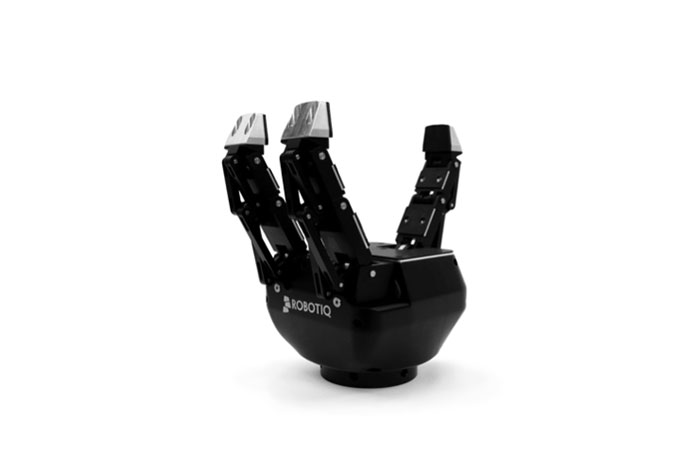
\includegraphics[width=\textwidth]{Img/three_finger_hand.jpg}
        \subcaption{三指欠驱动灵巧手}
        \label{fig:three_finger_hand}
    \end{minipage}
    \hfill
    \begin{minipage}[t]{0.48\textwidth}
        \centering
        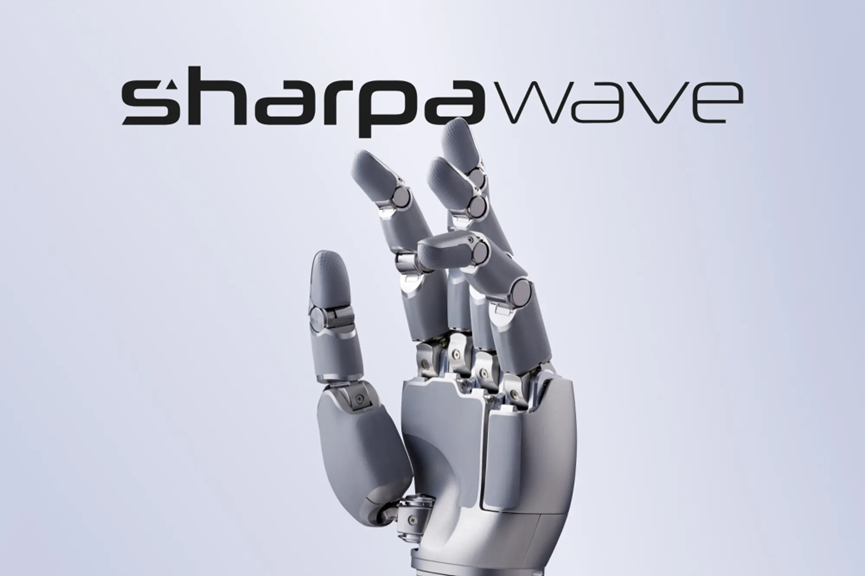
\includegraphics[width=\textwidth]{Img/sharpa_hand.png}
        \subcaption{SHARPA全驱动灵巧手}
        \label{fig:sharpa_hand}
    \end{minipage}
    \caption{不同类型的灵巧手}
    \label{fig:dexterous_hands}
\end{figure}

在机器人操作领域，传统工业机器人多采用单一的两指或三指夹爪，仅能完成简单的抓取、搬运等结构化任务，难以适应人类生活和复杂非结构化环境中的泛化需求。相比之下，仿生灵巧手（Dexterous Hand）具备高度的自由度和丰富的运动学特征，能够复刻人类的各种精细化操作（如捏、拧、插接、工具使用等）。因此，基于灵巧手的灵巧操作（Dexterous Manipulation）已成为当前具身智能领域最重要、也最具挑战性的研究前沿之一。

尽管多自由度灵巧手在硬件层面已具备执行复杂任务的物理基础，但如何为其赋予灵活的“智能大脑”仍面临巨大挑战。在现代人工智能的发展范式中，数据是驱动模型涌现强大泛化能力的最核心燃料。面对灵巧手极高的状态空间维度与复杂的物理交互模态，高度依赖数据的端到端学习方法已成为解决灵巧操作难题的主流路线。然而，训练具身大模型需要海量且高质量的专家数据。与唾手可得的互联网文本和图像不同，真实物理世界的灵巧操作数据获取成本高，数据质量参差不齐，导致当前具身智能领域正面临严峻的“数据荒”。研发可靠的遥操作（Teleoperation）系统，将人类专家的运动精准、便捷地重定向（Retarget）到真实硬件上，是一种有效提高灵巧操作数据采集效率和质量的方法。

正如\citet{BlackK-RSS-25}所述，具身大模型最为关键的两个方面是数据质量和训练范式（Training Recipe）。在通过遥操作系统获取高质量的专家数据后，如何高效利用这些数据并制定科学的训练范式，成为了具身模型迈向真机部署不得不解决的一个重要问题。对于比较前沿的灵巧操作控制策略算法，如基于动作分块的Transformer架构（ACT）、视觉-语言-动作模型（VLA）、世界模型（World Model）等，如何针对不同的架构的特性，来选择合适的数据与训练策略，是成功部署的关键所在。此外，真机部署还需要克服推理延迟、多源传感器数据对齐等“最后一公里”问题。

综上所述，面对具身智能领域的数据获取瓶颈与模型部署难题，本文致力于开发一套基于遥操作的便捷且高精度的灵巧操作数据采集平台。使用该系统获取了高质量专家数据之后，本文进一步探索了前沿架构的训练范式，并在同一实验平台上初步部署了$\pi_{0.5}$策略模型，实现了技术链路的闭环，为后续具身模型算法的研究与落地打下基础。

\section{研究现状}
本节将对灵巧操作的数据采集与策略模型研究现状进行综述。
\subsection{灵巧操作的数据采集研究}
一般来说，灵巧操作系统由机械臂和灵巧手两部分组成，由于他们的自由度差异很大（机械臂一般为 6--7 自由度，而全驱灵巧手自由度可达20个以上），获取这两部分专家数据的方法也存在较大差异。总体来说，机械臂数据采集方法相对成熟，而灵巧手数据采集方法则多种多样，尚未形成统一的主流方法。

实验室中最为常见、成熟的机械臂数据采集方法是使用同构主从机械结构，即通过一个与真实硬件结构相同的主设备来控制从设备。这种方法在机械臂数据采集中非常常见，如著名的\citet{Zhao-RSS-23}中开源的ALOHA系统，该方法具有低成本、双臂协同能力强、操作直观等优点。在末端执行器方面，\citet{Si-RSS-24}制作了一个具有四指的同构主从设备，可完成多种复杂的化学实验操作。然而，随着自由度的增加，同构主从设备的设计和制造难度迅速增长，且操作方法变得非常困难，导致其在全驱灵巧手数据采集中的应用受限。

\begin{figure}[htb]
    \centering
    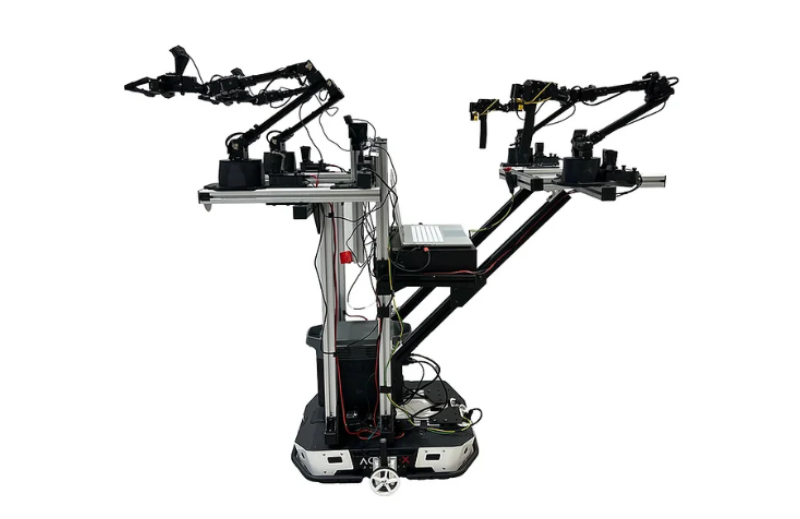
\includegraphics[width=0.55\textwidth]{Img/aloha.jpg}
    \caption{ALOHA同构主从机械臂遥操作系统}
    \label{fig:aloha}
\end{figure}

为缓解同构主从结构在高自由度灵巧手场景下的硬件复杂性，研究者开始采用外骨骼式主端进行遥操作数据采集。外骨骼系统通常佩戴在操作者手部或手臂上，通过机械结构、传感器或视觉追踪模块捕获人体手腕与手指运动，并进一步将其重定向到机器人灵巧手或臂手系统。相比完全同构的机械主手，该方法更贴近人的自然操作方式，适合采集高自由度、多接触的灵巧操作示教数据，且稳定性高。例如，\citet{pmlr-v270-yang25d}提出的ACE系统利用视觉-外骨骼结构实现了低成本、跨平台的灵巧遥操作，可支持不同类型的机器人手和夹爪。然而，外骨骼方法非常依赖于动作重定向算法和硬件人体工学设计，研发周期长，泛用性有限。

与外骨骼主端类似，数据手套等可穿戴设备也通过直接采集操作者手部运动来获取灵巧操作数据，但其通常不依赖刚性机械连杆对手指运动进行约束，而是通过惯性传感器、弯曲传感器或视觉追踪模块估计人手姿态。例如Manus等商业数据手套可以实时获取操作者手指弯曲状态和手腕位姿，并进一步通过逆运动学（IK）求解并使用重定向方法映射到机器人灵巧手的关节空间。相比外骨骼系统，数据手套具有更好的便携性和穿戴舒适性。例如，\citet{zheng2026egoscale}提出的EgoScale中就使用Manus数据手套获取手部数据。此外，数据手套便于扩展获取触觉等多模态信息，具有进一步发展的潜力。然而，由于数据手套采集到的是人体手部运动而非机器人本体动作，该类方法仍然需要解决不同人手与数据手套、数据手套与灵巧手之间的动作重定向问题。

\begin{figure}
    \centering
    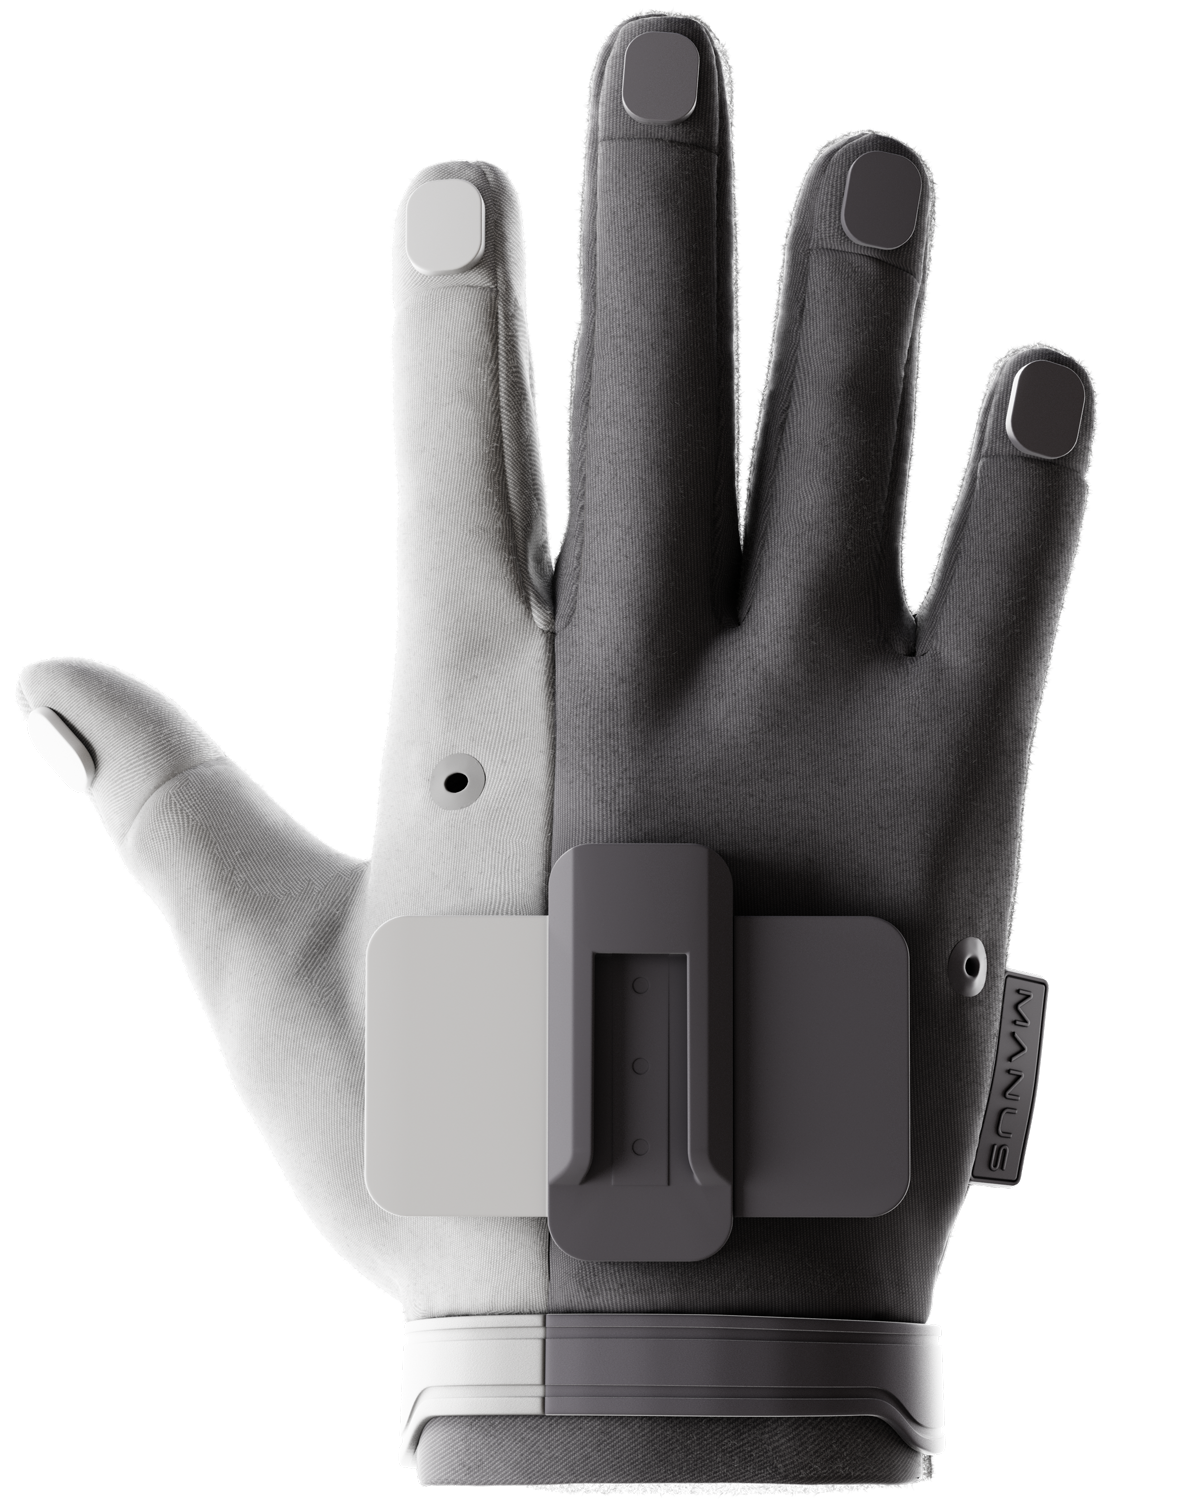
\includegraphics[width=0.3\textwidth]{Img/manus_glove.png}
    \caption{MANUS Metagloves Pro数据手套}
    \label{fig:manus_glove}
\end{figure}

进一步地，随着消费级 VR/AR 设备手部追踪与透视显示能力的提升，研究者开始探索不依赖专用机械主端、外骨骼或数据手套的轻量化遥操作采集方式。该类方法通常利用 VR/AR 头显获取操作者的头部、手腕和手指运动，并通过逆运动学求解或动作重定向将其映射到机器人本体，同时借助第一视角或立体视觉反馈提高操作者的空间感知能力。相比外骨骼和数据手套，基于 VR/AR 的方法部署成本更低、穿戴负担更小，且更容易适配不同机械臂、灵巧手和移动操作平台。例如，\citet{pmlr-v270-iyer25a}提出的 OPEN TEACH 系统基于Meta Quest 3 实现了多种机器人平台上的实时遥操作，并验证了其采集数据可用于灵巧和接触丰富任务的策略学习。然而，这类方法仍然面临手部追踪遮挡、视觉反馈延迟、缺少真实力触觉反馈以及人体动作到机器人动作重定向误差等问题，其可靠度、精度和操作手感有待提升。

\begin{figure}[htb]
    \centering
    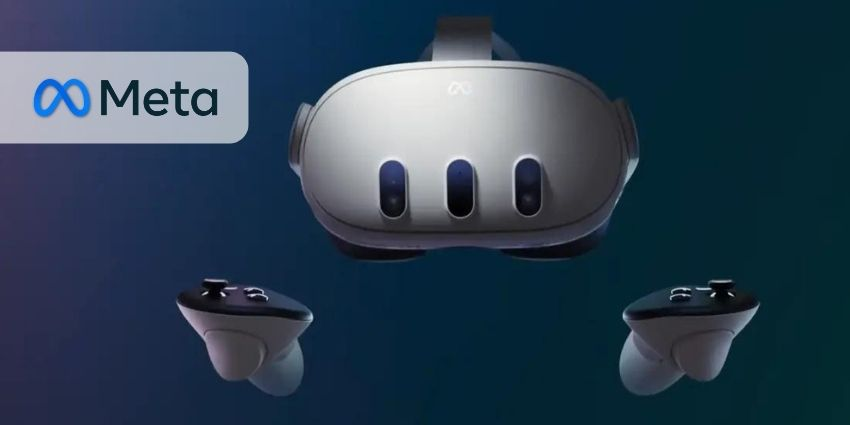
\includegraphics[width=0.5\textwidth]{Img/meta_quest_3.jpg}
    \caption{Meta Quest 3 VR数采套装}
    \label{fig:meta_quest_3}
\end{figure}

除上述依赖遥操作接口的方法外，最新研究进一步尝试直接从人类操作视频中获取机器人可用的示教信息。该类方法不要求操作者使用机械主端、外骨骼、数据手套或VR设备，而是通过普通相机或RGB-D相机记录人类完成任务的过程，并从视频中估计人体运动、手部姿态、物体状态或关键交互轨迹，再将其转化为机器人可执行的操作计划。代表性工作 OKAMI \citep{pmlr-v270-li25a} 仅利用单段RGB-D 人类示教视频，即可生成类人机器人的全身操作计划。该方法首先从视频中提取人体运动和物体交互信息，然后分别对身体动作和手部动作进行重定向，使机器人能够完成与视频中相似的操作任务。相比遥操作式数据采集，直接视频示教显著降低了数据获取门槛，并有潜力利用互联网上已有的大规模人类操作视频；但其仍然面临三维姿态估计误差、人体与机器人本体差异、接触状态恢复困难以及从观察到可执行动作的映射不确定性等挑战。

\subsection{灵巧操作的策略模型研究}
在策略模型方面，现有方法大致可以分为面向特定技能的小模型和面向通用操作的大模型两类。前者通常针对特定任务设计网络结构、奖励函数和仿真环境，并结合强化学习、模仿学习以及 sim-to-real 技巧实现真实部署。例如，HORA 通过在仿真中训练自适应控制器，实现了对多种未知物体的手内旋转泛化\citep{qi2022hora}；后续的转笔工作进一步结合仿真强化学习、真实轨迹回放和少量真实数据微调，使机器人能够对多种笔状物体完成动态旋转\citep{wang2025penspin}。此外，ALOHA 工作中提出的 ACT 框架采用条件变分自编码器和动作分块机制，从少量双臂示教数据中学习精细操作策略，并在多种双臂任务上表现出较好的泛化能力\citep{Zhao-RSS-23}。这类方法的优势在于控制频率高、训练目标明确、真实部署相对稳定，但其泛化通常仍局限于相近物体、相似场景或预定义任务族。

相比之下，近年来的研究重点逐渐转向面向通用操作的具身大模型，主要包括视觉-语言-动作模型（Vision-Language-Action Model, VLA）和世界模型（World Model）两条路线。VLA 方法通常将视觉观测、语言指令和机器人动作统一到同一模型中：视觉编码器负责提取场景和物体状态，语言模型提供任务语义和高层先验，动作则被表示为离散 token、连续动作块或 flow matching 目标进行预测。RT-2 首先展示了将互联网规模视觉语言知识迁移到机器人控制中的可行性\citep{zitkovich2023rt2}，OpenVLA 进一步开源了大规模 VLA 模型，并验证了其在真实机器人任务中的迁移与微调能力\citep{kim2025openvla}。Physical Intelligence 的 $\pi$ 系列则代表了近期 VLA 的快速演进：$\pi_0$ 采用视觉-语言-动作 flow 模型实现通用机器人控制\citep{BlackK-RSS-25}，$\pi_{0.5}$ 通过多机器人数据、网页数据和语义子任务预测增强开放世界泛化能力\citep{physicalintelligence2025pi05}，$\pi^{*}_{0.6}$ 进一步结合真实部署经验、在线采样和专家干预提升长程任务性能\citep{physicalintelligence2025pi06}，最新的 $\pi_{0.7}$ 则引入更丰富的多模态上下文条件以提升模型的可控性和跨本体迁移能力\citep{physicalintelligence2026pi07}。

然而，现有 VLA 仍主要依赖视觉、语言和本体状态，对于遮挡下的接触、滑移、柔性形变以及微小装配误差等信息建模不足。为弥补这一缺陷，触觉信息正逐渐成为灵巧操作中的重要模态。例如 Sharpa 的 CraftNet 将视觉、触觉、语言和动作建模为 VTLA 框架，并强调通过高密度触觉阵列提升末端精细操作能力\citep{sharpa2026craftnet}。这表明未来的灵巧操作策略可能不再只依赖视觉语言先验，而需要进一步融合触觉等接触模态，以提升接触丰富任务中的鲁棒性和精度。

除直接预测动作的 VLA 外，世界模型也成为具身策略模型的重要方向。与 VLA 直接从当前观测和任务条件生成动作不同，世界模型更强调学习环境状态在动作条件下的时序演化规律，即建模“如果执行某个动作，未来场景会如何变化”。NVIDIA 提出的 DreamZero 将预训练视频生成模型扩展为 World Action Model，通过联合预测未来视频帧和机器人动作来建模环境动态，从而探索利用世界模型实现零样本策略泛化的可能性\citep{ye2026dreamzero}。这类方法的优势在于能够从连续视频中学习物体运动、接触变化和任务进展等动态信息，因此有潜力利用大量无动作标签的人类或机器人视频数据。

总体来看，具身大模型普遍遵循预训练与微调相结合的训练范式，但不同架构对数据的需求并不相同。VLA 模型通常需要包含视觉观测、语言指令和机器人动作的配对数据，其中视觉提供物体和场景状态，语言提供任务目标和语义约束，动作数据则提供可执行的控制监督；因此，其性能很大程度上依赖大规模、高质量且覆盖多任务的机器人示教数据。触觉增强的 VTLA 模型在此基础上还需要同步的触觉信号，以补充视觉难以观测的接触状态。相比之下，世界模型的预训练可以更多利用大规模视频数据学习通用时空和物理先验，再通过机器人交互数据进行动作条件化微调，使其具备从预测未来状态到生成动作的能力。由此可见，数据的模态组成、动作标注质量以及跨任务覆盖范围，直接决定了不同策略模型的训练方式和可部署能力。

因此，本文将围绕高质量灵巧操作数据获取与策略模型部署两方面展开：前者为不同模型提供可靠的真实示教数据基础，后者则用于验证所采集数据在VLA策略框架中的实际使用价值。

\section{论文结构安排}

本文围绕灵巧操作数据采集平台构建、遥操作重定向方法以及 $\pi_{0.5}$ 策略真机部署三部分展开。全文主要内容安排如下：

第一章为绪论。首先介绍具身智能与灵巧操作的发展背景，说明高质量真实示教数据对灵巧操作策略学习的重要意义；随后从数据采集方法和策略模型两方面综述相关研究现状，分析现有方法在高自由度灵巧手数据获取、动作重定向和真机策略部署中的主要挑战；最后给出本文的章节组织结构。

第二章介绍灵巧操作数据采集平台的构成。该章从硬件和软件两方面说明本文实验平台的设计：硬件部分包括天机 Marvin 双臂、WUJI HAND 灵巧手、HTC Vive Tracker 动捕系统、MANUS 数据手套、多视角相机和脚踏开关等模块；软件部分基于 ROS 2 Jazzy 构建，负责设备驱动、数据同步、任务调度和 rosbag 记录。该章为后续遥操作控制和数据集构建提供系统基础。

第三章介绍数据采集系统中的数学原理。该章重点说明如何将操作者的 Tracker 位姿和 MANUS 手部骨架数据转换为机器人可执行的关节命令。其中，机械臂部分通过坐标系变换、人体到机器人末端位姿映射、逆运动学求解和臂角搜索获得连续稳定的关节角；灵巧手部分则通过手部骨架标准化和模型约束优化完成从人手姿态到 WUJI HAND 20 维关节空间的重定向。

第四章介绍 $\pi_{0.5}$ 策略模型的真机部署。该章首先概述 $\pi_{0.5}$ 的视觉-语言-动作模型结构和 Flow Matching 动作生成机制；随后说明本文平台中的动作空间、视觉输入、数据集构建和训练配置；最后给出真机实验结果，并对抓取位置错误、手部高度偏低和动作输出退化等失败现象进行分析，讨论数据质量和光照条件对策略性能的影响。

附录部分补充正文中不便展开的配置和推导细节，包括 Tracker 与机械臂遥操作中的预定义刚体变换参数、齐次最小二乘与 SVD 的数学推导，以及 $\pi_{0.5}$ 真机部署和策略训练的关键配置表。
